\documentclass{standalone}

\usepackage{tikz}
\usepackage{tikz-qtree}


%% TODO: finish diagram, do at home for better workflow integration

\begin{document}
\begin{figure}
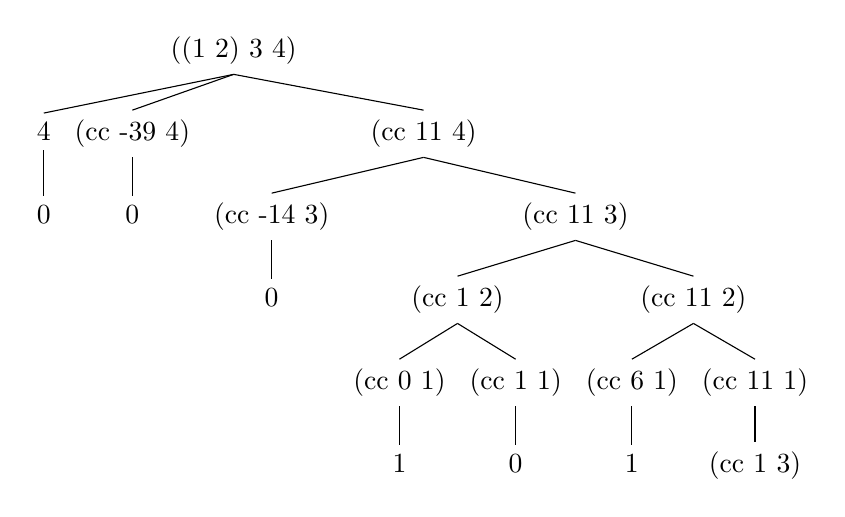
\begin{tikzpicture}
    %\tikzset{grow'=right,level distance=64pt}
    %\tikzset{execute at begin node=\strut}
    %\tikzset{every tree node/.style={anchor=base west}}
    \Tree 
        [.\node {((1 2) 3 4)};
            [.\node {4}; 0 ]
            [.\node {(cc -39 4)}; 0 ]
            [.\node {(cc 11 4)};
                [.\node {(cc -14 3)}; 0 ]
                [.\node {(cc 11 3)}; 
                    [.\node {(cc 1 2)}; 
                        [.\node {(cc 0 1)}; 1 ]
                        [.\node {(cc 1 1)}; 0 ]
                    ]
                    [.\node {(cc 11 2)};
                        [.\node {(cc 6 1)}; 1 ]
                        [.\node {(cc 11 1)};
                            [.\node {(cc 1 3)}; 
                            ]
                        ]
                    ] 
                ]
            ]
        ]
\end{tikzpicture}
\caption{SICP: Figure 2.6}
\end{figure}

%\begin{tikzpicture}
%\Tree [.CP [.NP \node(wh){what}; ]
%           [.C$'$ [.I did ]
%                  [.\node[draw]{IP};
%                    [.NP [.Det the ] [.N cat ] ]
%                    [.VP [.V sit ]
%                        [.PP [.P on ]
%                            [.\node[draw]{NP};
%                                [.NP [.Det a ] [.N book ] ]
%                                [.PP [.P about ] [.NP \node(t){$t$}; ] ] ] ] ] ] ] ]
%    \draw[semithick,->] (t)..controls +(south west:5) and +(south:5)..(wh);
%\end{tikzpicture}
\end{document}
